%====================================================================================
\section{Riesgo moral}
%====================================================================================

\begin{frame}{Desarrollo temporal del riesgo moral}
	\begin{center}
		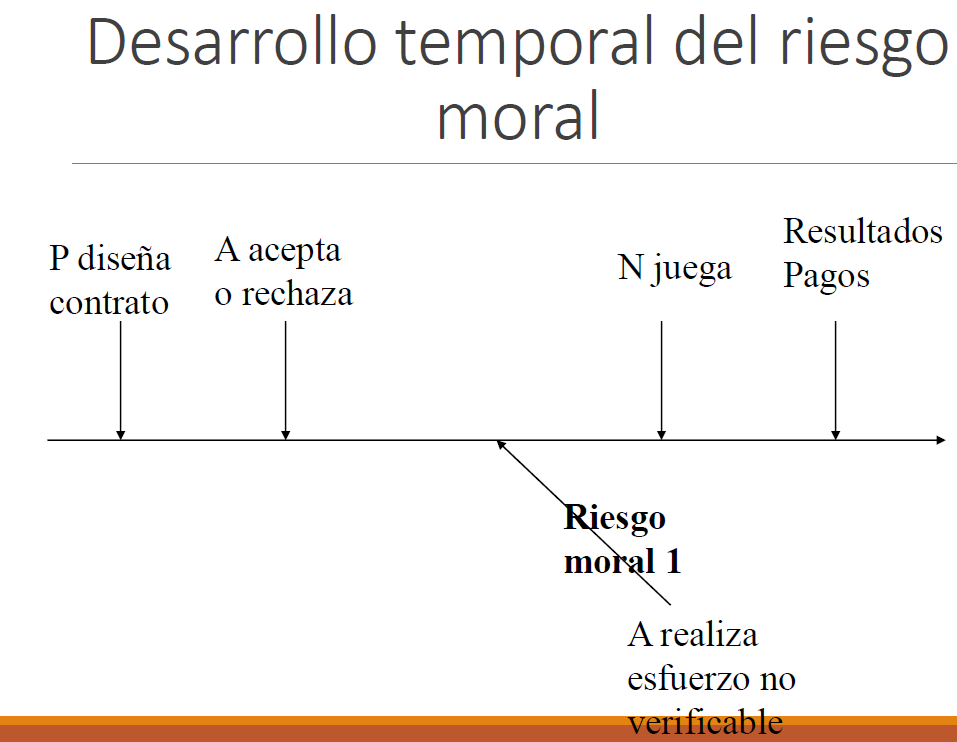
\includegraphics[width = 0.9\linewidth]{figures/fig_00.png}
	\end{center}
\end{frame}
%------------------------------------------------
\begin{frame}{Ejemplo}
	Una empresa de catering contrata un cocinero para el diseño y realización de menús de alta calidad. El propietario de la empresa es neutral ante el riesgo. La función de utilidad del cocinero es
		$$U(w, e) = \sqrt{w} -v(e)$$
	Si el cocinero realiza un trabajo de alta calidad, $v=36$ y si realiza un trabajo rutinario $v=16$. La utilidad de reserva del cocinero es 114. Si el cocinero realiza un trabajo de alta calidad, la probabilidad de éxito es $2/3$ mientras que si realiza un trabajo rutinario la probabilidad de éxito disminuye a $1/3$.\\
	
	El éxito implica unos beneficios de 60 000 para la empresa mientras que el fracaso implica un nivel de beneficios de 30 000.
\end{frame}
%------------------------------------------------
\begin{frame}{Ejemplo}
	\begin{enumerate}[a)]
		\item Suponiendo que el esfuerzo es observable por parte de la empresa, hallar el contrato óptimo.
		\item Si la empresa no puede observar el esfuerzo del trabajador, ¿le conviene a la empresa aplicar la solución a) para que el trabajo sea de calidad alta?
	\end{enumerate}
\end{frame}
%------------------------------------------------
\begin{frame}{Con Riesgo Moral}
		\begin{itemize}
			\item Si el principal neutral al riesgo ofrece al agente un contrato basado en un pago fijo, el agente decidirá realizar un esfuerzo mínimo
			\item El principal elegirá aquel contrato que remunere al agente exactamente por el esfuerzo que va a realizar
			\item El pago del agente no puede depender del esfuerzo realizado, sino del resultado obtenido (observado por el principal ).
		\end{itemize}
\end{frame}
%------------------------------------------------
\begin{frame}{Con Riesgo Moral}
	Si el principal quiere inducir el esfuerzo alto:
		\begin{itemize}
			\item Tiene que dar al agente incentivos a esforzarse.
			\item El agente tiene que estar mejor cuando su esfuerzo es alto que cuando su esfuerzo es bajo
		\end{itemize}
	Si el principal quiere inducir el esfuerzo bajo:
		\begin{itemize}
			\item no es necesario poner ningún tipo de incentivo para inducir el esfuerzo bajo.
			\item El contrato que el principal ofrece al agente es el mismo que cuando el esfuerzo es observable: se ofrece siempre el salario de reserva para el esfuerzo bajo.
		\end{itemize}
\end{frame}
%------------------------------------------------
\begin{frame}{Programa de Riesgo Moral}
	Con información asimétrica , el principal debe estudiar qu é esfuerzo desea incorporar el agente, pero no puede introducirlo en los términos del contrato.\\
	
	Dado que el agente decide en la última etapa cuánto esfuerzo realiza, si el principal desea cierto nivel de esfuerzo del agente, debe darle incentivos (=pagar según los resultados obtenidos.
\end{frame}
%------------------------------------------------
\begin{frame}{Programa de Riesgo Moral}
	Si $e$ principal desea un esfuerzo e, se debe satisfacer:
		$$ e \in \arg \M \left\lbrace \sum p_i(\hat{e})u\left[ w\left( x_i\right) \right] - v\left( \hat{e}\right) \right\rbrace $$
	Esta condición ( restricción de incentivos) refleja el hecho que una vez aceptado el contrato y dado que el esfuerzo no es verificable, el agente elige el esfuerzo que maximiza su función objetivo.
\end{frame}
%------------------------------------------------
\begin{frame}{Programa de Riesgo Moral}
	Luego de conocer el contrato, el agente decide si lo acepta o no.\\
	
	Igual que con información simétrica, esto se presenta por la restricción de participación:
		$$\sum p_i(e)u\left[ w\left( x_i\right) \right] - v\left( e\right) \geq \underline{U}$$
\end{frame}
%------------------------------------------------
\begin{frame}{Programa de Riesgo Moral}
	Por tanto, el problema (o programa) del principal es de la forma:
		\begin{align*}
			& \text{Max } \quad \sum_{1}^{n}p_i(e)B\left[x_i - w\left( x_i\right) \right] \\
			& \begin{array}{ll}
				\text{s.a: } & \sum p_i(e) u\left[ w\left( x_i\right) \right] - v\left( e \right) \geq \underline{U}\\[0.3cm]
							 & e \in \arg \M \sum p_i(\hat{e})u\left[ w\left( x_i\right) \right] - v\left( \hat{e}\right)
			\end{array}
		\end{align*}
\end{frame}
%------------------------------------------------
\begin{frame}{Programa de Riesgo Moral}
	Es decir:
		\begin{itemize}
			\item el contrato debe ofrecer una utilidad mayor que la utilidad de reserva (restricción de participación, o de racionalidad individual).
			\item el contrato debe ofrecer una utilidad más alta para el esfuerzo más alto (restricción de incentivos).
			\item para que el contrato que induce el esfuerzo más alto sea óptimo, el principal debe de obtener más beneficio que cuando induce el esfuerzo bajo (restricción adicional.
		\end{itemize}
\end{frame}
%------------------------------------------------
\begin{frame}{Contrato Óptimo Compatible con los Incentivos que induce el esfuerzo alto.}
	Deben cumplirse las siguientes restricciones:
		\begin{itemize}
			\item \textbf{Restricción de participación}: : el agente tienen que obtener una utilidad superior a su utilidad de reserva, si no, no aceptará el contrato.
			\item \textbf{Restricción de incentivos}: : el agente tiene que tener incentivos a realizar el nivel de esfuerzo e que se intenta inducir con el contrato.
			\item \textbf{Restricción Adicional}: : el principal debe de obtener más beneficio induciendo el esfuerzo alto que induciendo el esfuerzo bajo.
		\end{itemize}
\end{frame}
%------------------------------------------------
\begin{frame}{Modelo sencillo: agente que elige entre dos esfuerzos}
	Caso más sencillo : el agente sólo tiene la posibilidad de escoger entre dos niveles de esfuerzo:
		\begin{itemize}
			\item Nivel $e^H =$ situación en la que el agente trabaja
			\item Nivel $e^L =$ el esfuerzo es bajo
		\end{itemize}
\end{frame}
%------------------------------------------------
\begin{frame}{Supuestos:}
	\begin{enumerate}
		\item El esfuerzo puede tomar únicamente dos valores:
			\begin{itemize}
				\item Por tanto:
					\begin{gather*}
						e \in \left\lbrace e^H, e^L\right\rbrace\\
						v\left( e^H\right) > v\left( e^L\right)
					\end{gather*}
			\end{itemize}
		\item El principal es neutral. Concretamente:
			$$B\left( x -w \right) = x-w$$
		\item El conjunto de resultados se ordena de peor a mejor:
			$$x_1 < x_2 < \ldots < x_n$$
	\end{enumerate}
\end{frame}
%------------------------------------------------
\begin{frame}{Supuestos:}
	\begin{enumerate}[4]
		\item Como el resultado no depende sólo del esfuerzo del agente, sino que tiene un componente aleatorio, el resultado es a su vez una variable aleatoria:
			\begin{gather*}
				p_{i}^{H} = p_i\left( e^H\right) = p\left( x = x_i \mid e^H\right) ; \sum p_{i}^{H} = 1\\
				p_{i}^{L} = p_i\left( e^L\right) = p\left( x = x_i \mid e^L\right) ; \sum p_{i}^{L} = 1
			\end{gather*}
		\item Para todo resultado, las probabilidades de que se obtengan dichos resultados cuando el esfuerzo es alto (o bajo) son mayores que cero:
			$$0 < p_i < 1 , \forall i$$
	\end{enumerate}
\end{frame}
%------------------------------------------------
\begin{frame}{Supuestos:}
	\begin{enumerate}[6]
		\item Dominancia estocástica de primer orden: es más fácil obtener resultados malos cuando se trabajo poco que cuando se trabaja duro.\\
		Por tanto, si eliminamos el mejor resultado:
			$$\sum_{i=1}^{k}p_i\left( e^H\right) < \sum_{i=1}^{k}p_i\left( e^L\right) , \forall k = 1, \ldots, n-1$$
	\end{enumerate}
\end{frame}
%------------------------------------------------
\begin{frame}{Contrato óptimo si el principal desea esfuerzo bajo}
	En este caso no existirá el problema de riesgo moral, ya que bastará con hacer un pago fijo.
		$$w^L = u^{-1}\left[ \overline{U} + v\left(e^L \right) \right]$$
	El agente escogerá el esfuerzo bajo, ya que es el que maximiza su utilidad.
		$$u\left( w^L\right) - v\left( e^L\right) > u\left( w^L\right) - v\left( e^H\right) $$
\end{frame}
%------------------------------------------------
\begin{frame}{Contrato óptimo si el principal desea esfuerzo alto}
	Para conseguir que el principal realice el esfuerzo alto, el esquema salarial debe cumplir la siguiente condición (restricción de incentivos):
		\begin{gather*}
			\sum p_{i}^{H}u\left[w(x_i) \right] - v\left( e^H\right) \geq \sum p_{i}^Lu\left[ w\left( x_i\right) \right] - v\left( e^L\right)\\
			\sum \left( p_{i}^{H} - p_{i}^{L}\right) u\left[ w\left( x_i\right) \right] \geq v\left( e^H\right) - v\left( e^L\right) 
		\end{gather*}
	El agente elige el esfuerzo $e^H$, si la esperanza de ganancia asociada a este esfuerzo es superior al costo que implica realizarlo.\\
	
	El esquema salarial debe lograr que el agente tenga interés en lograr el esfuerzo alto $e^H$.
\end{frame}
%------------------------------------------------
\begin{frame}{Contrato óptimo si el principal desea esfuerzo alto}
	Por lo tanto: para determinar el esquema salarial que consigue inducir en el agente el esfuerzo alto y proporciona máximos beneficios al principal, éste deberá resolver el siguiente problema:
		\begin{align*}
			& \text{Max } \quad \sum_{1}^{n}p_{i}^{H}\left[x_i - w\left( x_i\right) \right] \\
			& \begin{array}{ll}
				\text{s.a: } & \sum p_{i}^{H} u\left[ w\left( x_i\right) \right] - v\left( e^H \right) \geq \underline{U} \text{ R.P.}\\[0.3cm]
						     & \sum\left( p_{i}^{H} - p_{i}^{L}\right) u\left[ \left(x_i \right) \right] \geq v\left( e^H\right) - v\left( e^L\right)  \text{ R.I.}
			\end{array}
		\end{align*}
\end{frame}
%------------------------------------------------
\begin{frame}{Contrato óptimo si el principal desea esfuerzo alto}
	El Lagrangiano será:
		\begin{align*}
			L = & \sum_{1}^{n}p_{i}^{H}\left[x_i - w\left( x_i\right) \right]\\
				& \lambda \left\lbrace \sum p_{i}^{H} u\left[ w\left( x_i\right) \right] - v\left( e^H \right) - \underline{U} \right\rbrace +\\
				& \mu \left\lbrace \sum\left( p_{i}^{H} - p_{i}^{L}\right) u\left[ \left(x_i \right) \right] - v\left( e^H\right) + v\left( e^L\right) \right\rbrace 
		\end{align*}
	La CPO, para cada $i$:
		$$\frac{\partial L}{\partial w\left( x_i\right)} = 0 \rightarrow - p_{i}^{H}+\lambda p_{i}^{H}u^\prime \left[ w\left( x_i\right) \right] + \mu \left( p_{i}^{H} - p_{i}^{L}\right)u^\prime\left[ w\left( x_i\right) \right] =0$$
	O:
		\begin{gather*}
			\left[ \lambda p_{i}^{H} + \mu \left(p_{i}^{H} - p_{i}^{L} \right) \right]u^\prime \left[ w\left( x_i\right) \right] = p_{i}^{H}\\
			\frac{p_{i}^{H}}{u^\prime \left[ w\left( x_i\right) \right]} = \lambda p_{i}^{H} + \mu \left(p_{i}^{H} - p_{i}^{L} \right)
		\end{gather*}
\end{frame}
%------------------------------------------------
\begin{frame}{Contrato óptimo si el principal desea esfuerzo alto}
	Sumando las n ecuaciones:
		\begin{gather*}
			\sum \frac{p_{i}^{H}}{u^\prime \left[ w\left( x_i\right) \right]} = \lambda \sum p_{i}^{H} + \mu \sum \left(p_{i}^{H} - p_{i}^{L} \right)
		\end{gather*}
	La R.P. Está saturada
		$$\lambda = \sum \frac{p_{i}^{H}}{u^\prime \left[ w\left( x_i\right) \right]} > 0$$
\end{frame}
%------------------------------------------------
\begin{frame}{Propiedades del contrato óptimo}
	Reescribiendo las CPO:
		\begin{align*}
			\frac{p_{i}^{H}}{u^\prime \left[ w\left( x_i\right) \right]} &= p_{i}^{H} + \mu \sum \left( p_{i}^{H} - p_{i}^{L} \right)\\[0.3cm]
			\frac{1}{u^\prime \left[ w\left( x_i\right) \right]} &= \lambda + \mu \left( 1 - \frac{p_{i}^{L}}{p_{i}^{H}}\right) \\[0.3cm]
			u^\prime \left[ w\left( x_i\right) \right] &= \frac{1}{\lambda + \mu \left( 1 - \frac{p_{i}^{L}}{p_{i}^{H}}\right)} 
		\end{align*}
	Si $\mu = 0$, entonces:
		$$u^\prime \left[ w\left( x_i\right) \right]$$
	Lo que supondría que el salario sería constante, pero el esfuerzo elegido por el agente sería el menor, no el mayor. Por tanto, para inducir esfuerzo alto: $\mu \neq 0$
\end{frame}
%------------------------------------------------
\begin{frame}{Propiedades del contrato óptimo}
	¿Qué implica $\mu > 0$
		\begin{itemize}
			\item Que el riesgo moral tiene un costo positivo para el principal.
			\item Que los beneficios del principal son mayores cuando la información respecto al esfuerzo es simétrica, en comparación a una situación de riesgo moral.
			\item Que los pagos del agente varían en función al resultado.
		\end{itemize}
	Es decir:
		$$w\left( x_i\right) = \left(  u^\prime \right)^{-1} \left[ \frac{1}{\lambda + \mu \left( 1 - \frac{p_{i}^{L}}{p_{i}^{H}}\right)} \right] $$
	$\frac{p_{i}^{L}}{p_{i}^{H}}$ = ratios de verosimilitud.\\
	
	Cuanto menor sea el ratio, mayor será el pago, porque mayor será la señal de que el resultado procede de un esfuerzo alto
\end{frame}
%------------------------------------------------
\begin{frame}{Gráficamente}
	\begin{center}
		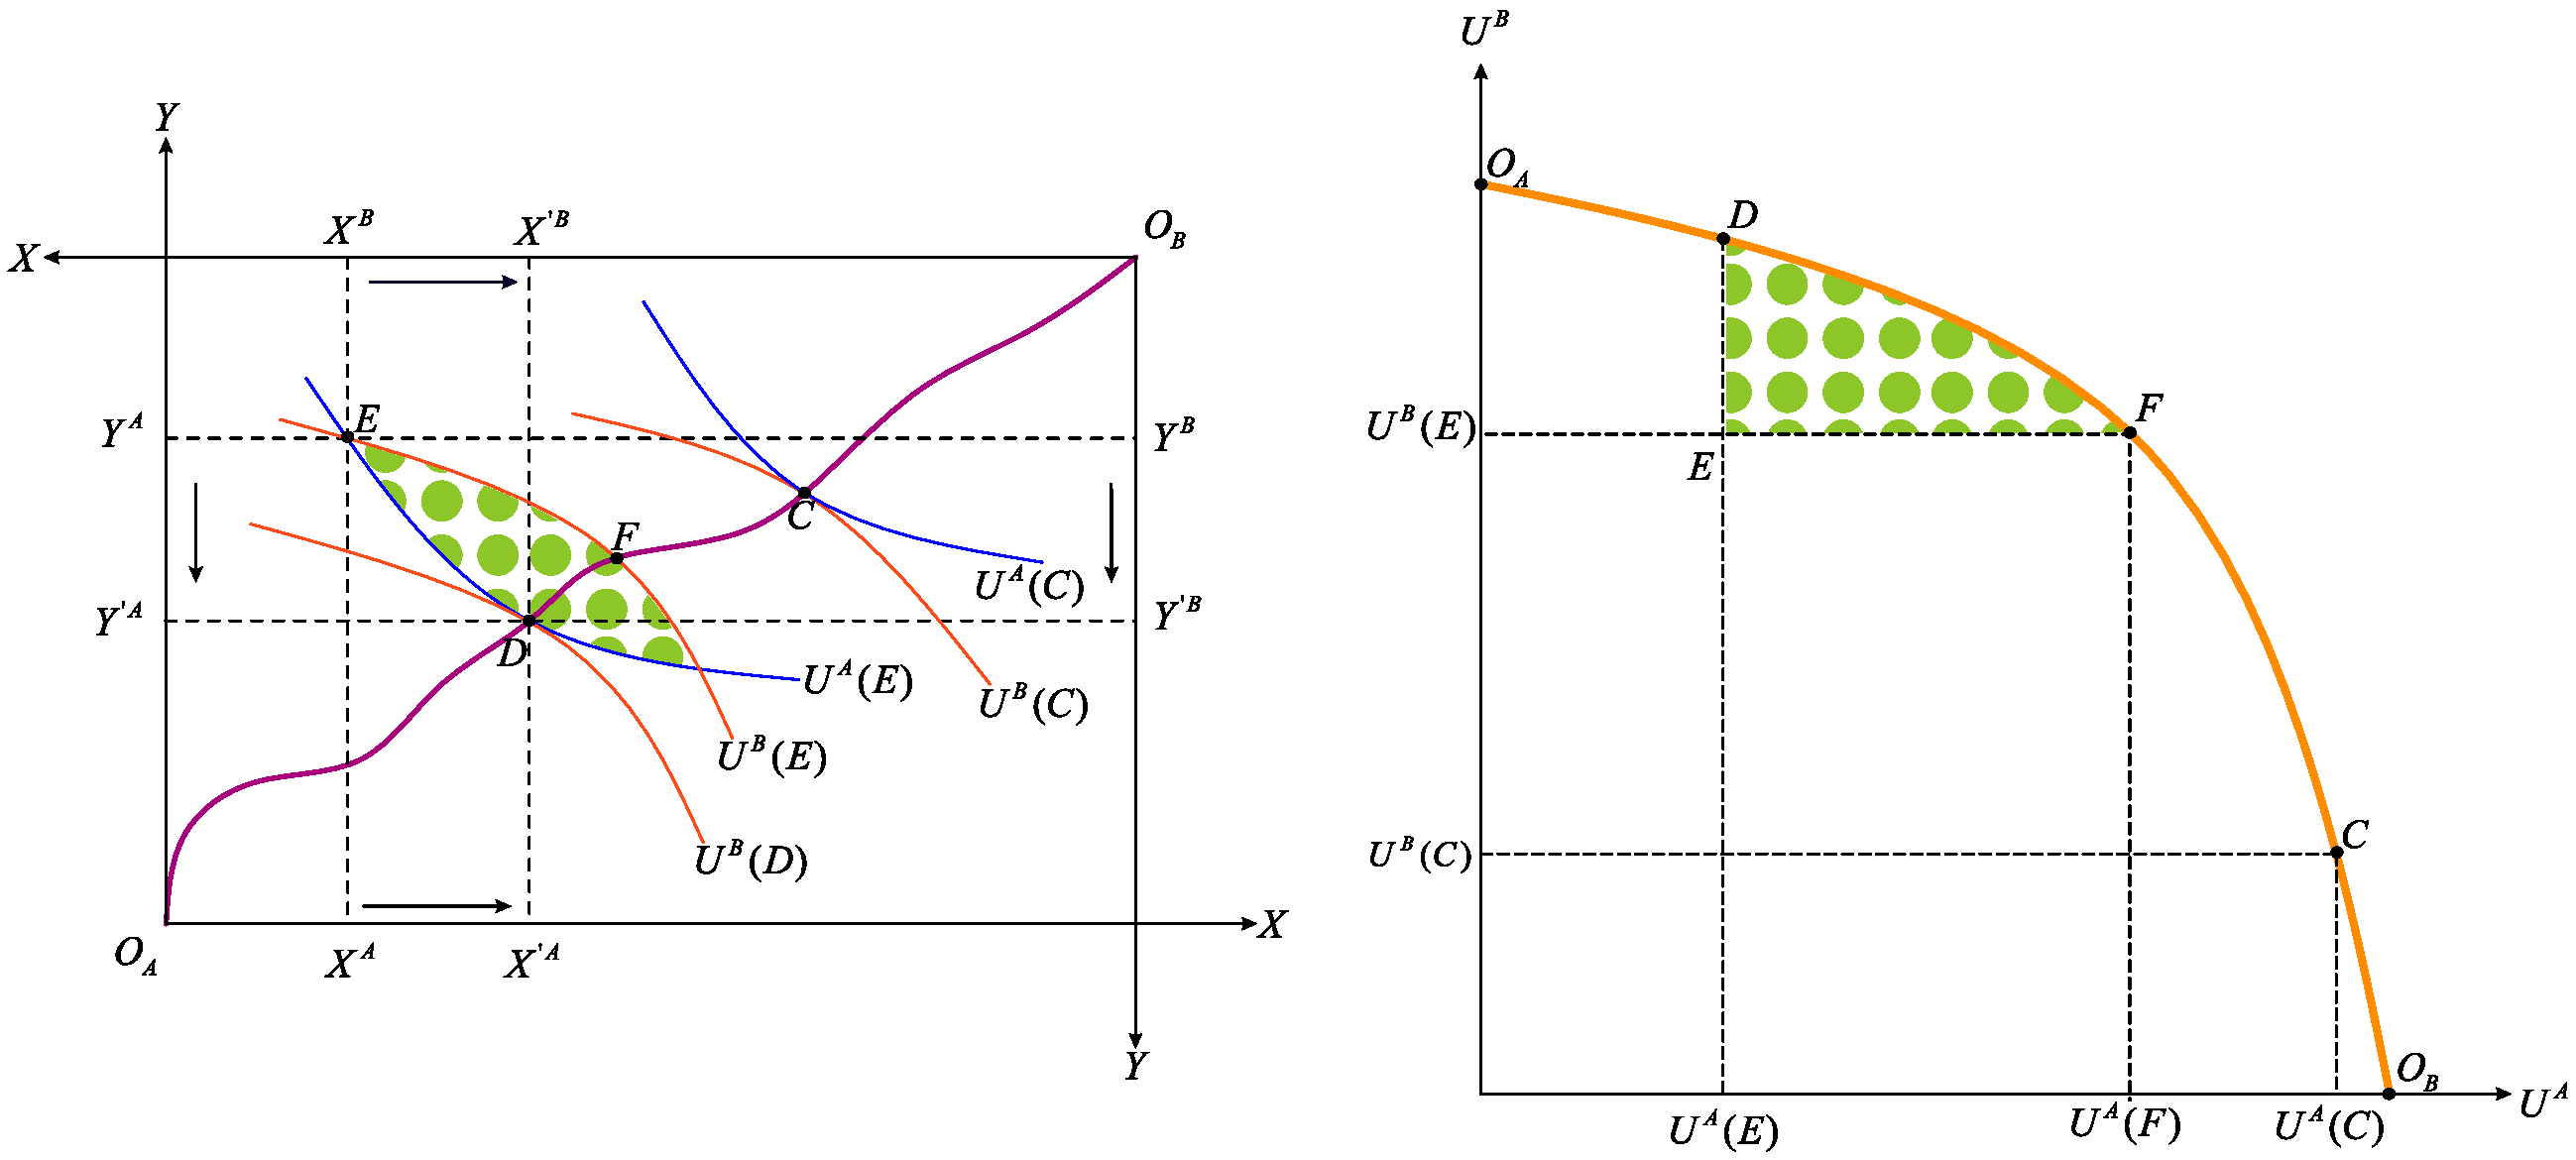
\includegraphics[width = 0.9\linewidth]{figures/fig_01.png}
	\end{center}
\end{frame}
%------------------------------------------------
\begin{frame}{Gráficamente}
	\begin{center}
		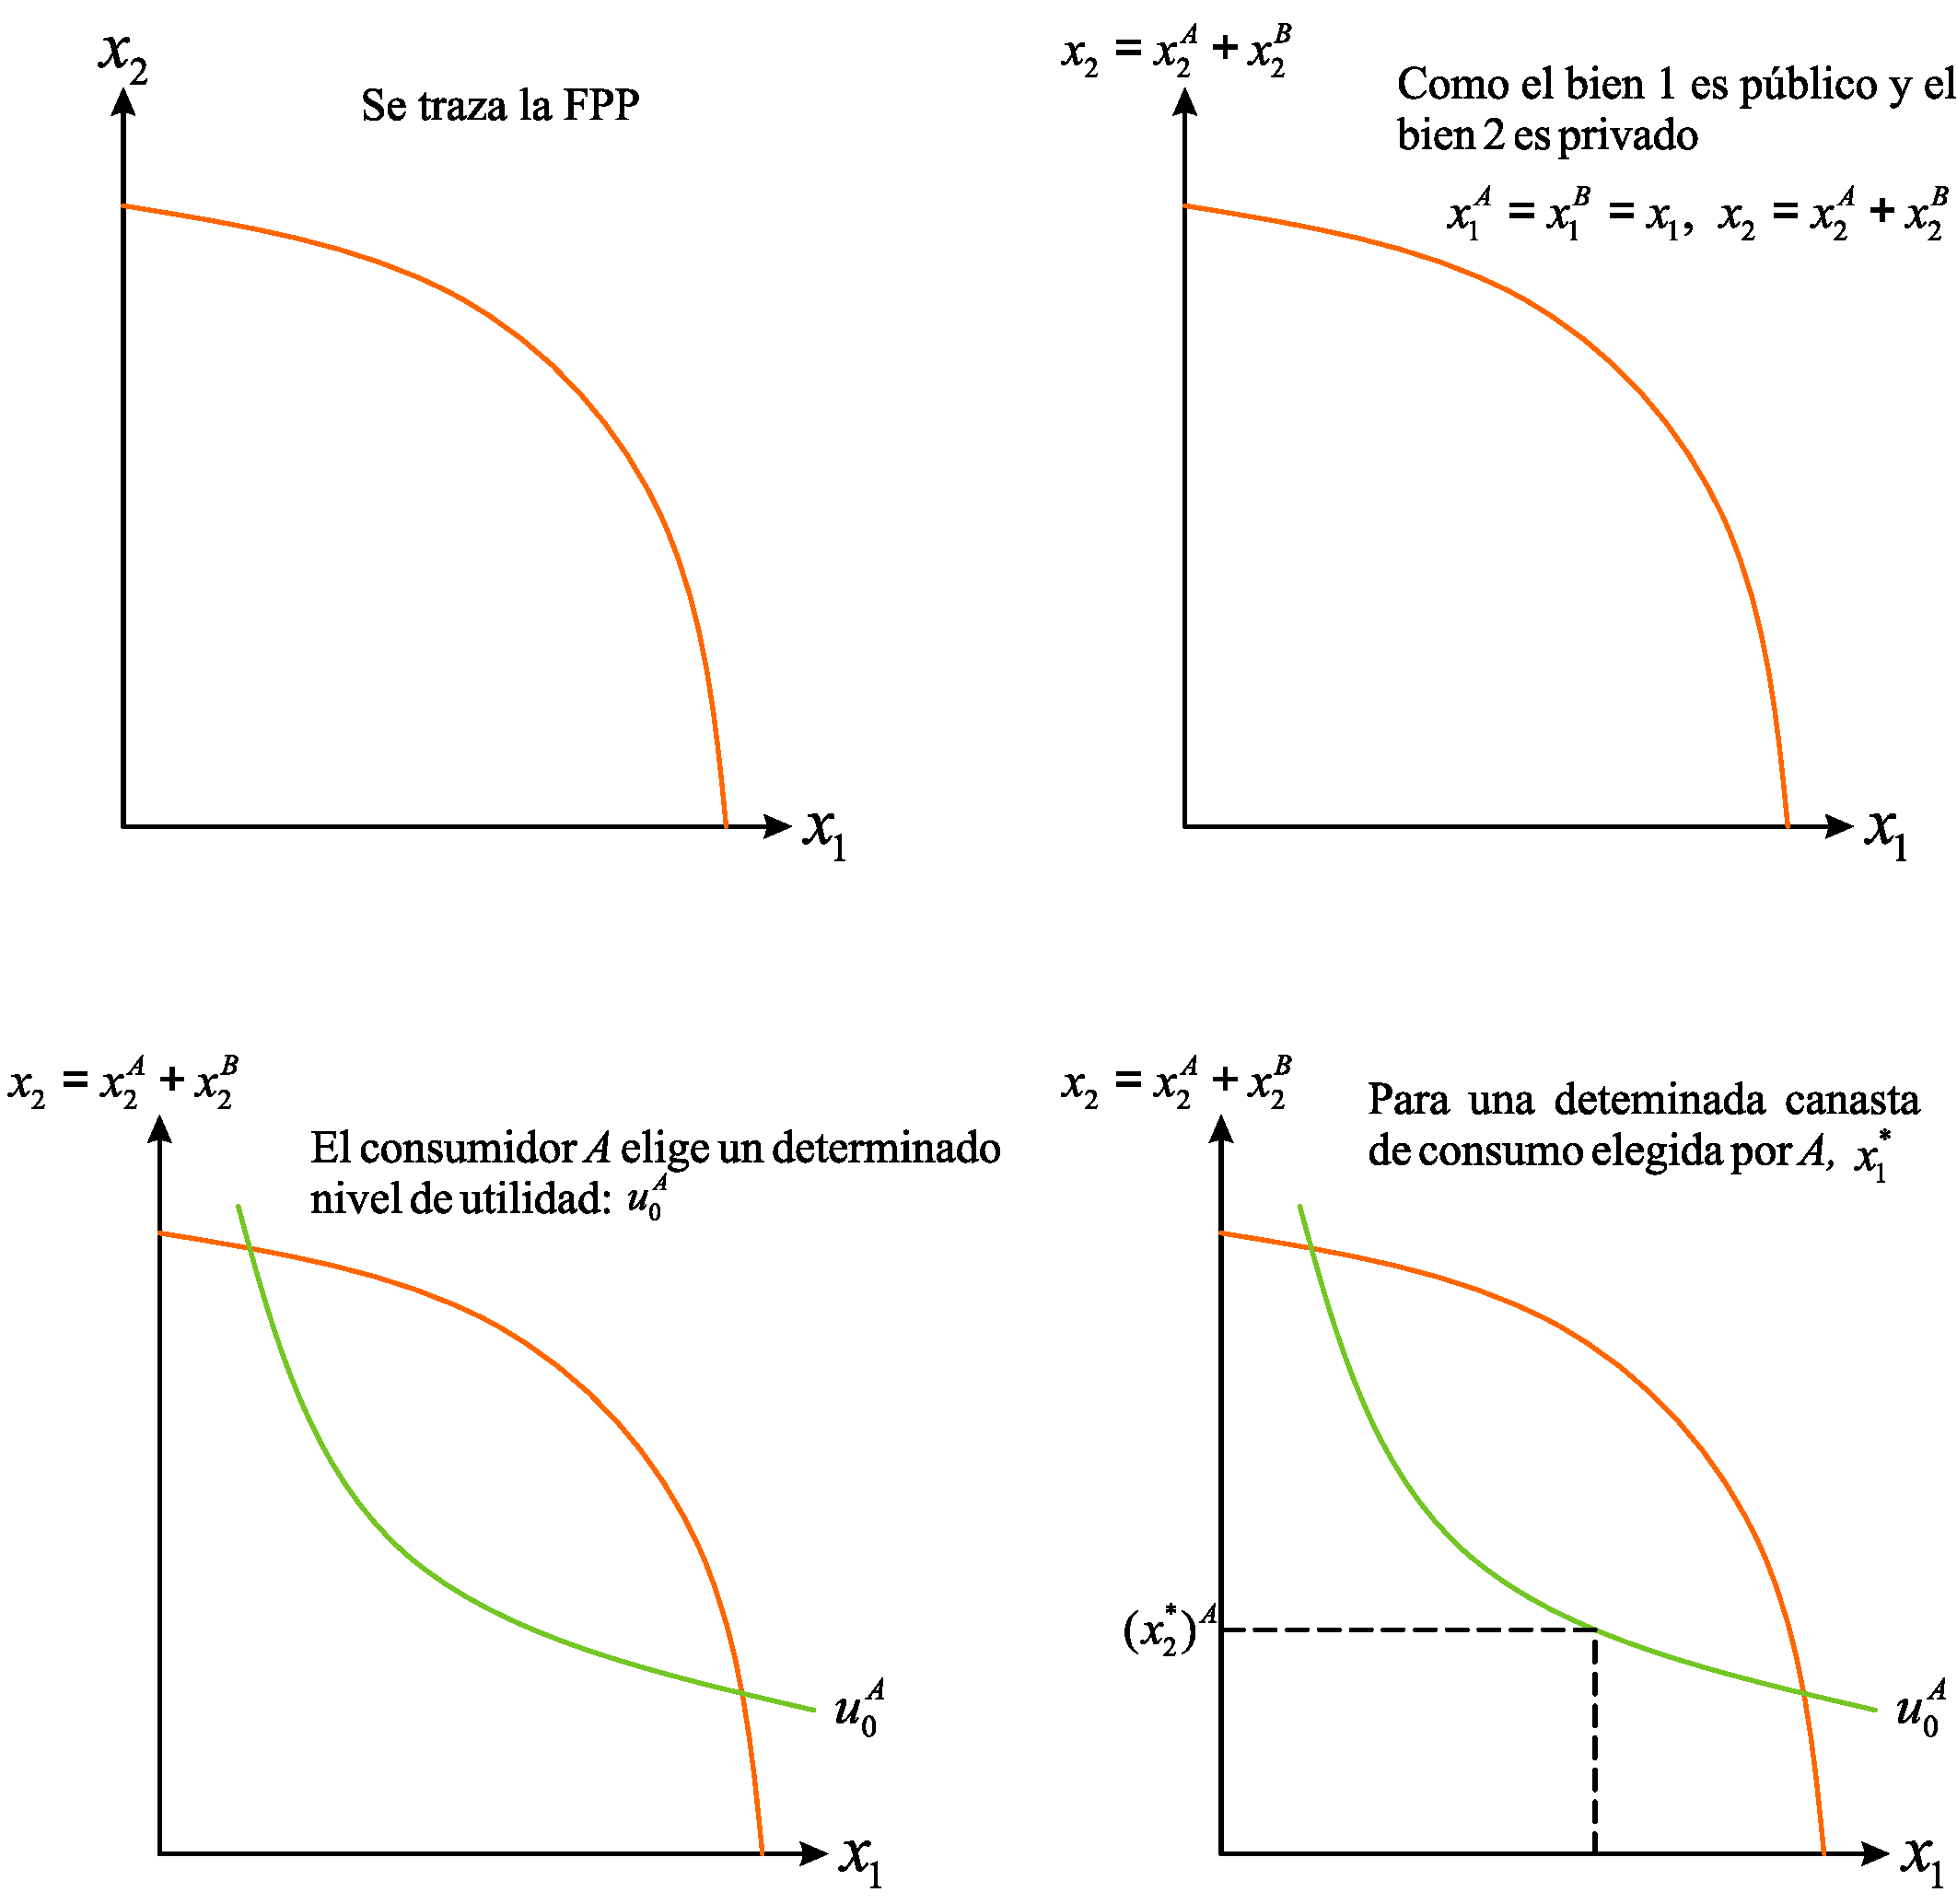
\includegraphics[width = 0.9\linewidth]{figures/fig_02.png}
	\end{center}
\end{frame}
%------------------------------------------------
\begin{frame}{Gráficamente}
	\begin{center}
		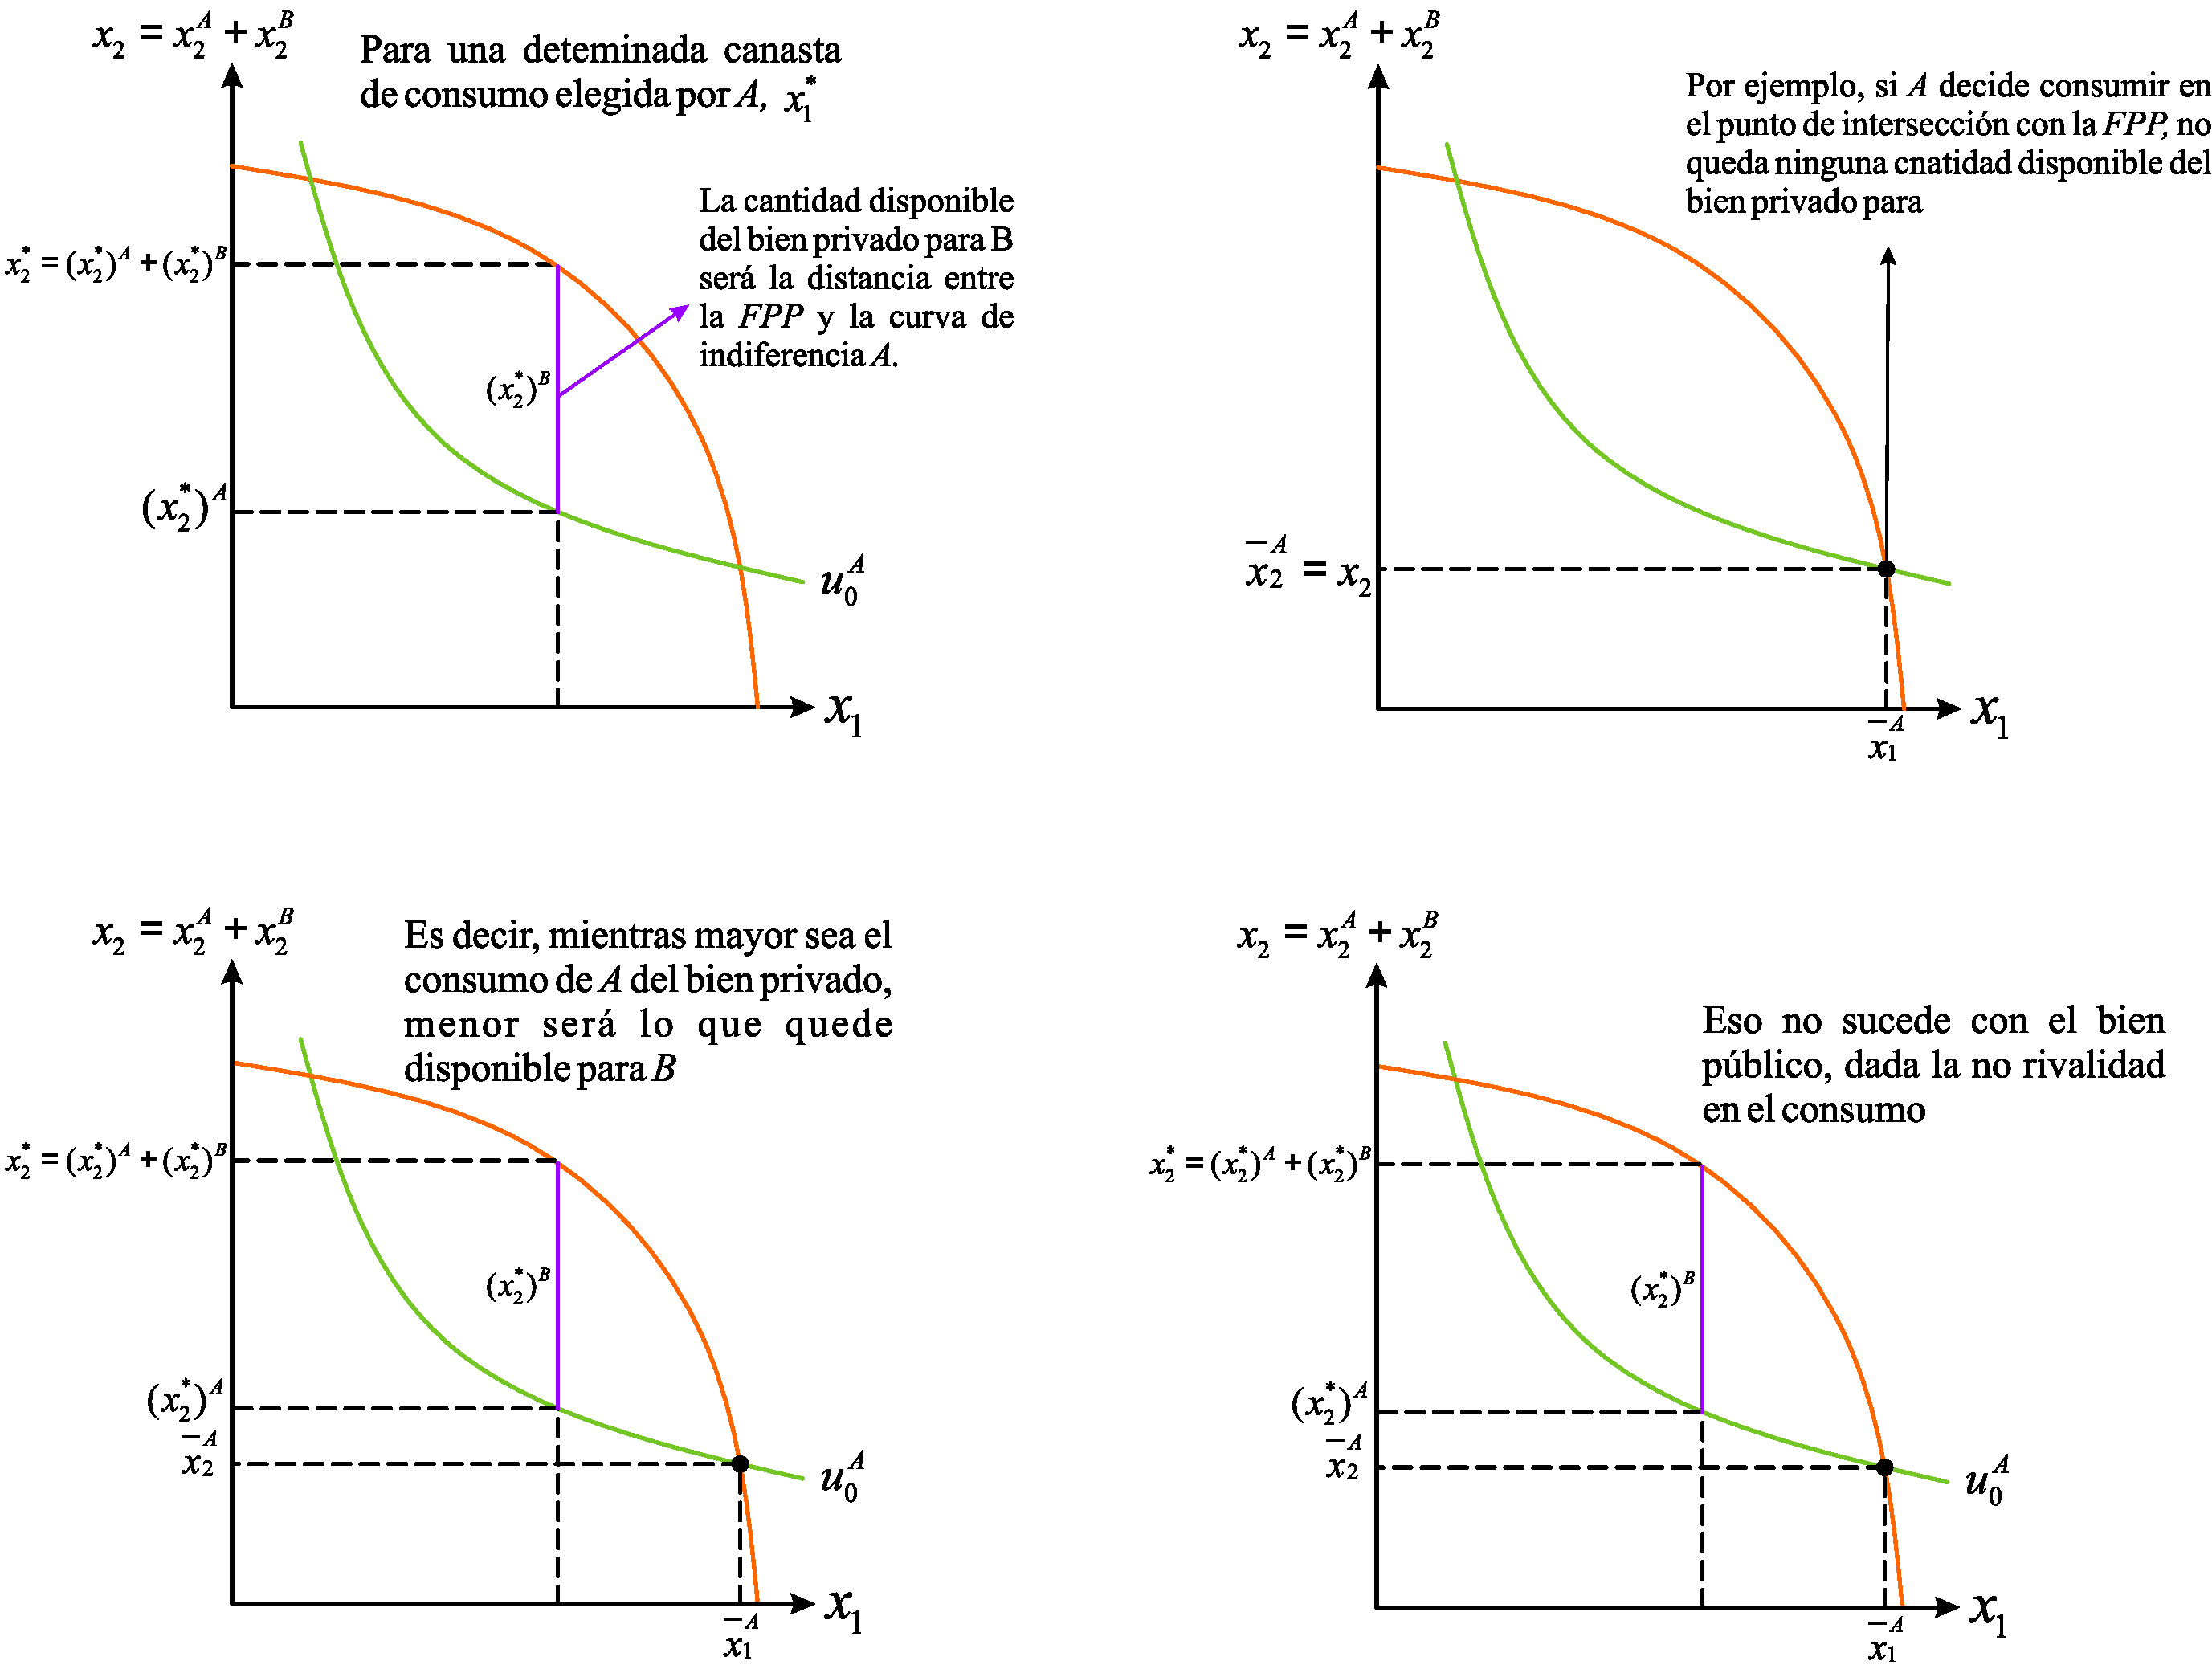
\includegraphics[width = 0.9\linewidth]{figures/fig_03.png}
	\end{center}
\end{frame}
%------------------------------------------------
\begin{frame}{Gráficamente}
	\begin{center}
		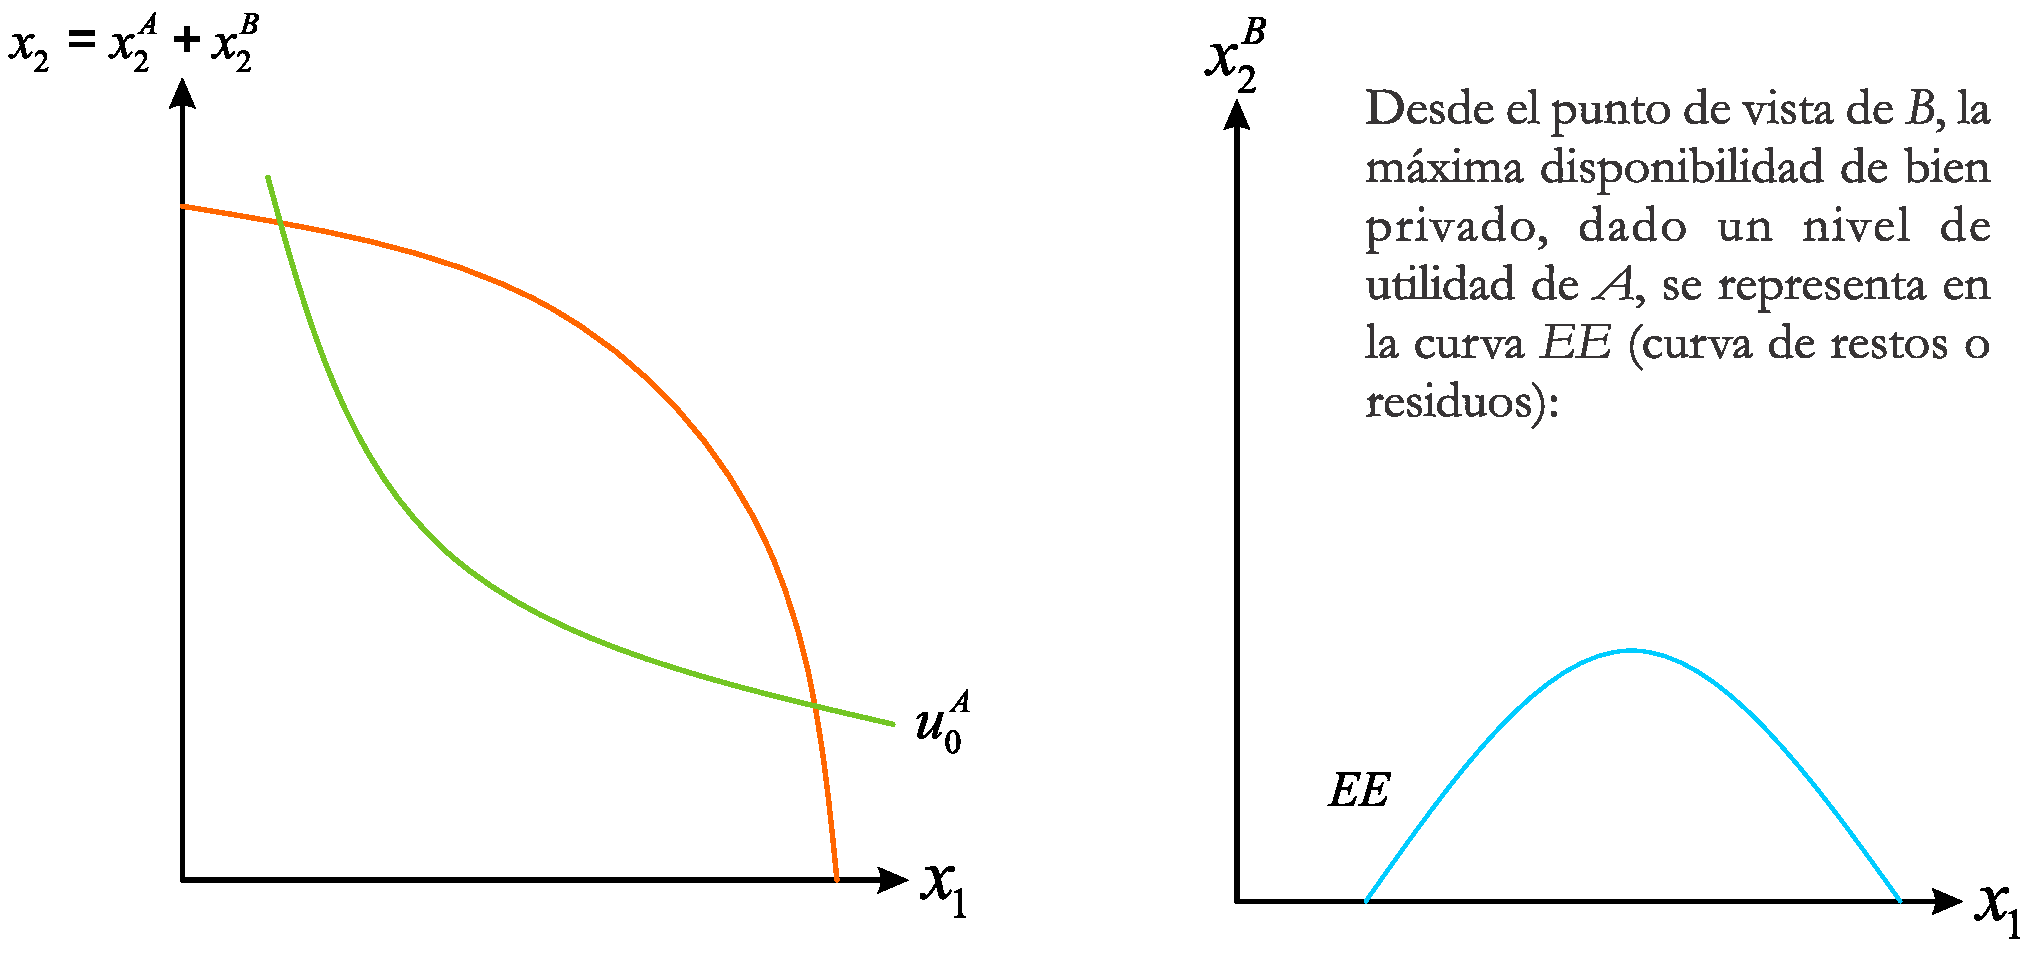
\includegraphics[width = 0.9\linewidth]{figures/fig_04.png}
	\end{center}
\end{frame}
%------------------------------------------------
\begin{frame}{Gráficamente}
	\begin{center}
		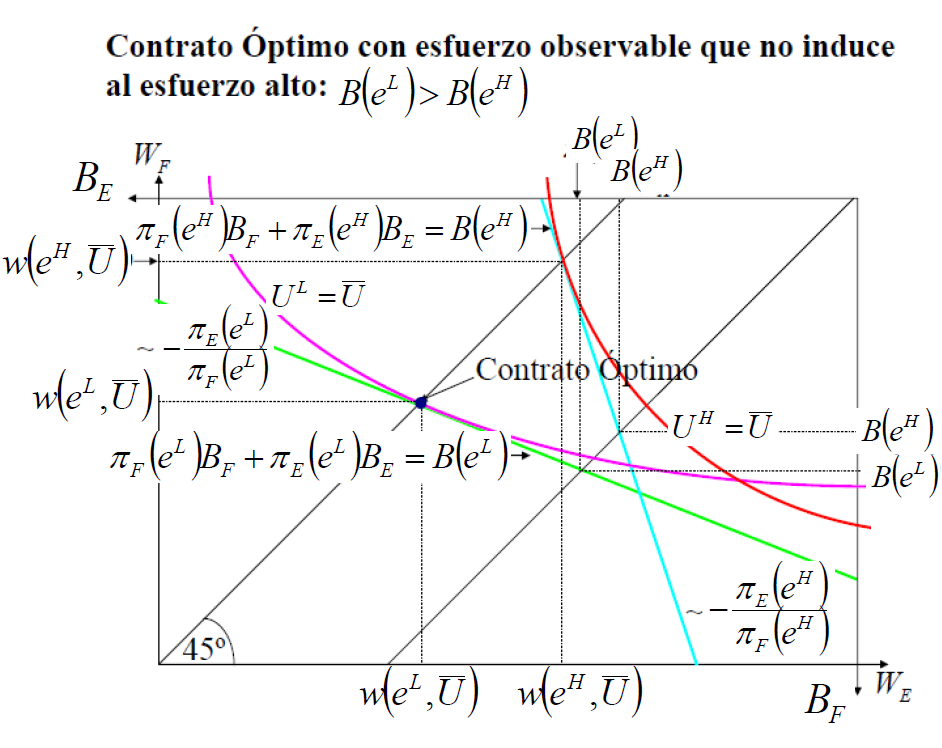
\includegraphics[width = 0.9\linewidth]{figures/fig_05.png}
	\end{center}
\end{frame}
%------------------------------------------------
\begin{frame}{Gráficamente}
	\begin{center}
		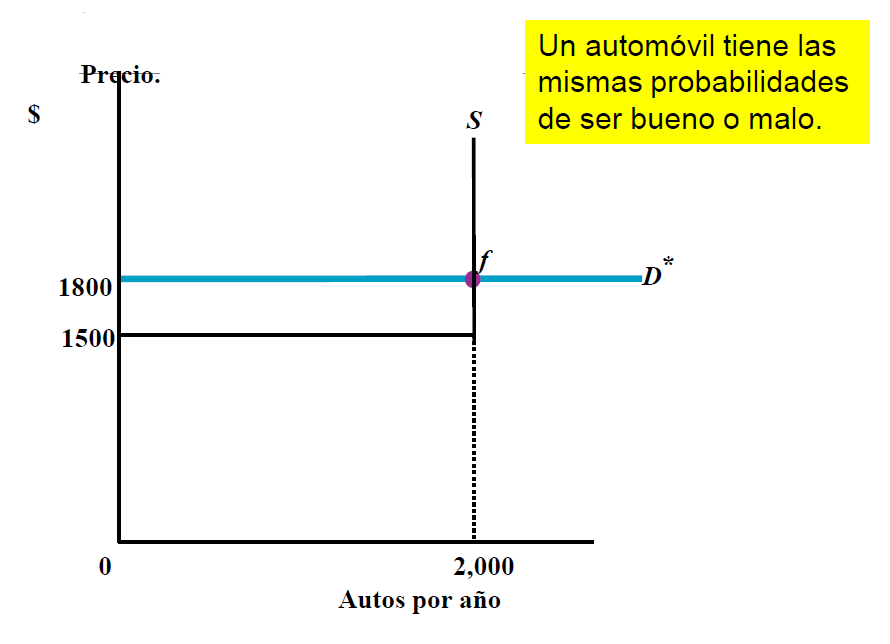
\includegraphics[width = 0.9\linewidth]{figures/fig_06.png}
	\end{center}
\end{frame}
%------------------------------------------------
\begin{frame}{Gráficamente}
	\begin{center}
		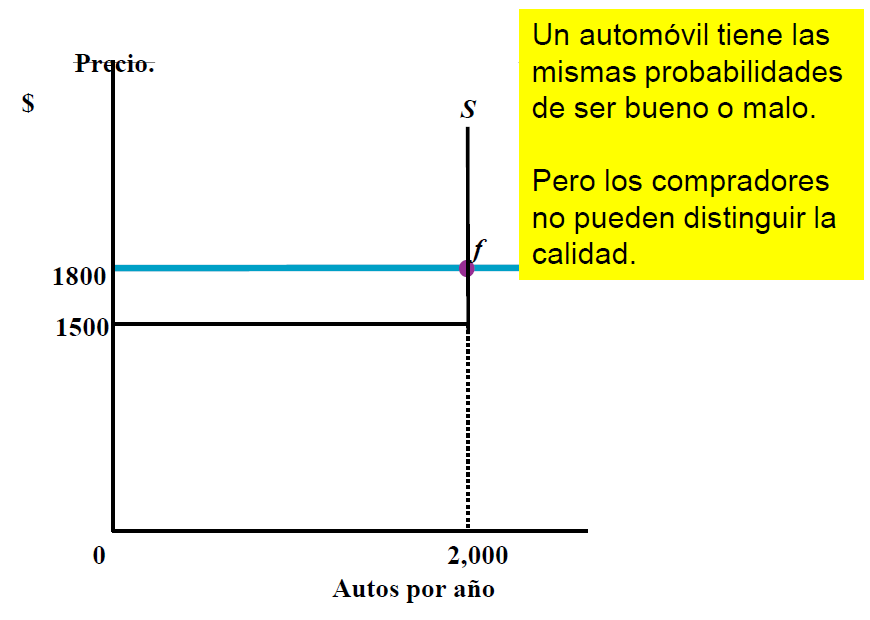
\includegraphics[width = 0.9\linewidth]{figures/fig_07.png}
	\end{center}
\end{frame}
%------------------------------------------------
\begin{frame}{Gráficamente}
	\begin{center}
		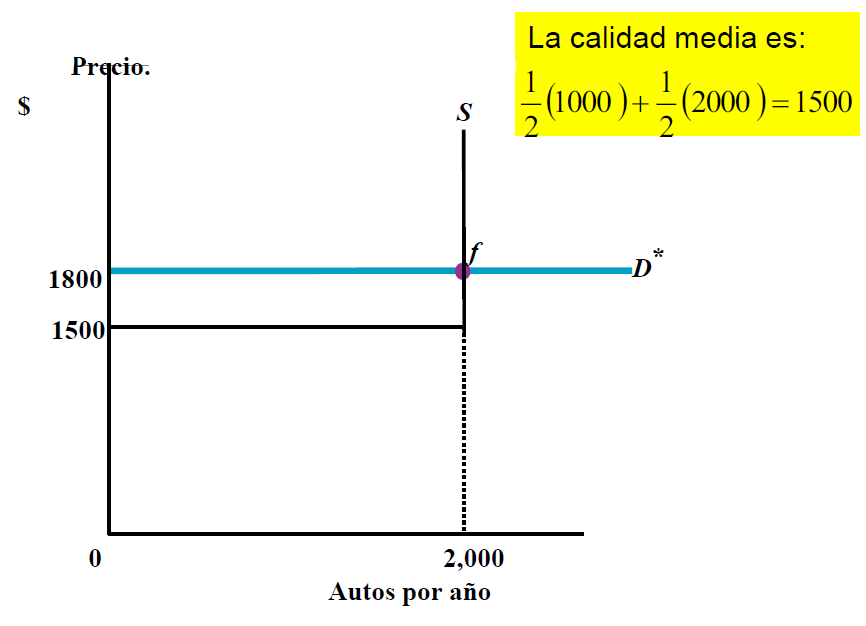
\includegraphics[width = 0.9\linewidth]{figures/fig_08.png}
	\end{center}
\end{frame}
%------------------------------------------------
\begin{frame}{Gráficamente}
	\begin{center}
		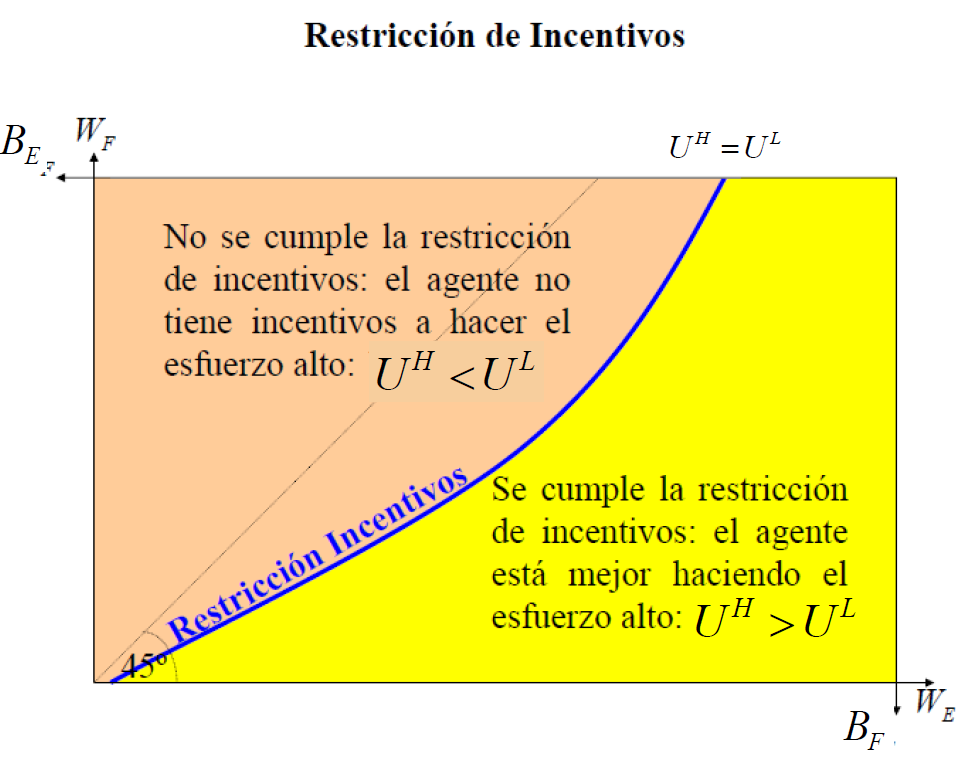
\includegraphics[width = 0.9\linewidth]{figures/fig_09.png}
	\end{center}
\end{frame}
%------------------------------------------------
\begin{frame}{Gráficamente}
	\begin{center}
		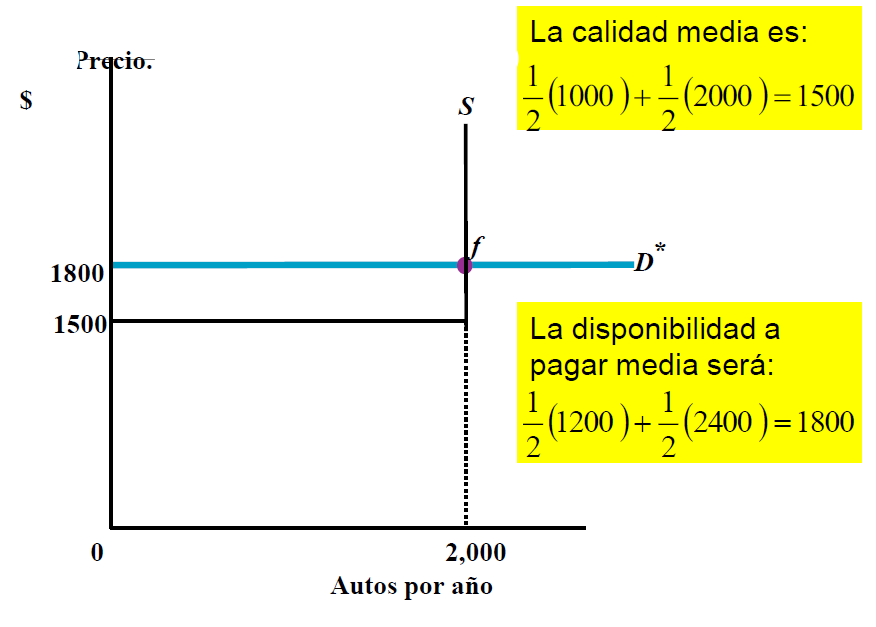
\includegraphics[width = 0.9\linewidth]{figures/fig_10.png}
	\end{center}
\end{frame}
%------------------------------------------------
\begin{frame}{Gráficamente}
	\begin{center}
		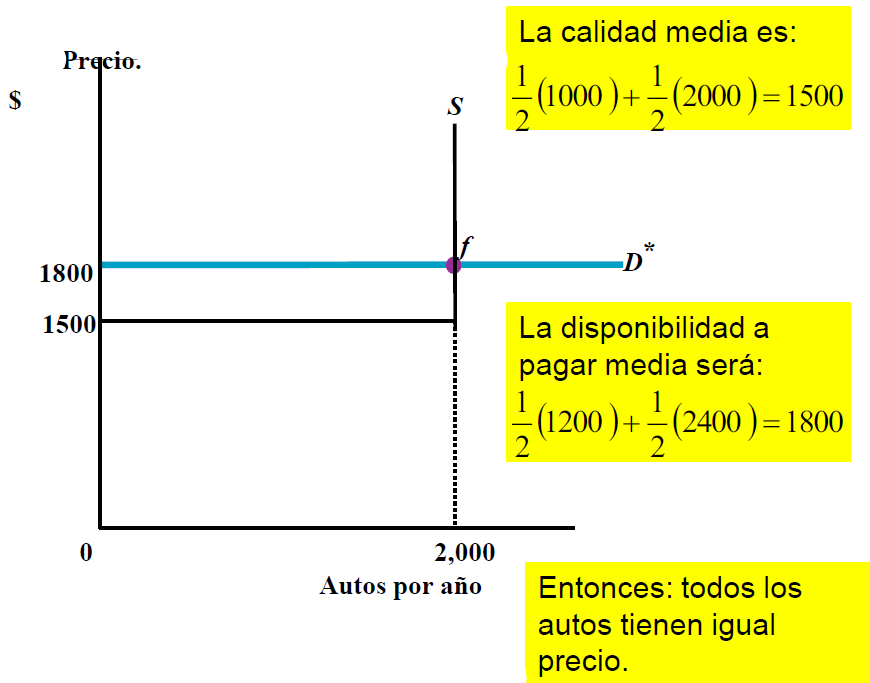
\includegraphics[width = 0.9\linewidth]{figures/fig_11.png}
	\end{center}
\end{frame}
%------------------------------------------------
\begin{frame}{Gráficamente}
	\begin{center}
		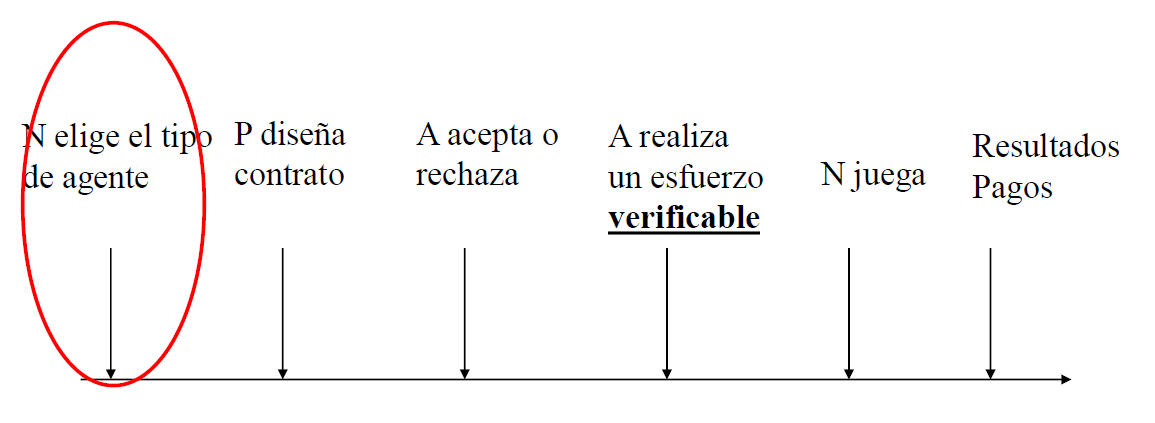
\includegraphics[width = 0.9\linewidth]{figures/fig_12.png}
	\end{center}
\end{frame}
%------------------------------------------------
\begin{frame}{Gráficamente}
	\begin{center}
		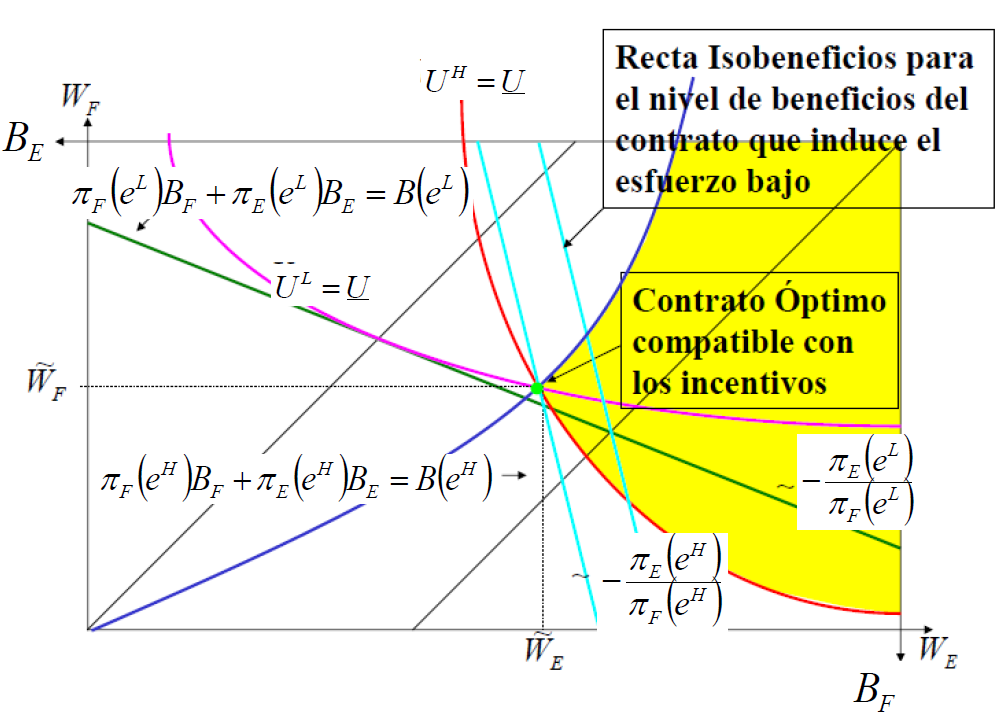
\includegraphics[width = 0.9\linewidth]{figures/fig_13.png}
	\end{center}
\end{frame}
%------------------------------------------------